\section{Experiments}
\label{sec:exp}

\subsection{Setup}
\label{sec:exp-setup}

\textbf{Hardware.} One server, 4$\times$Tesla V100-PCIE-32GB (Volta; fp16, no FlashAttention-2), 72 CPU cores, 125\,GB RAM. One GPU was occupied by an unrelated tenant during fleet runs; all fleet results use 3 GPUs and say so.

\textbf{Models.} Tier-1 salience: VadCLIP~\cite{vadclip} (scores replayed from our causally-computed per-clip score files; tier-1 cost is charged at its measured rate, Appendix~\ref{app:e0}). Narrator: Qwen2.5-VL-7B~\cite{qwen25vl}, fp16, SDPA attention (the stock triton/flash kernels do not run on Volta; Appendix~\ref{app:porting}), 8 frames/event, temperature 0.2. Verification/judging: the same model and InternVL2-8B~\cite{internvl} cross-family. Retrieval embeddings: bge-small-en~\cite{bge}. Baseline models: LLaVA-OneVision 0.5B/7B~\cite{llavaov} for ReKV~\cite{rekv}.

\textbf{Datasets.} UCF-Crime test (290 videos, 10.3\,h, 156 ground-truth anomaly events, 13 categories)~\cite{ucfcrime}; XD-Violence test (800 videos, 27.0\,h, 1{,}238 events, 6 categories)~\cite{xdviolence}; ShanghaiTech test (107 anomalous videos, 12 cameras, 194 events)~\cite{shanghaitech}. Generality arm: RVS-Ego (10 Ego4D videos, 120 questions, 9.6 stream-hours)~\cite{flashvstream}.

\textbf{Reproducibility.} Every experiment is a run directory with config, environment, code-state (commits + patches), data manifest, and cost accounting (Appendix~\ref{app:repro}).

\subsection{SMB: a surveillance memory benchmark}
\label{sec:exp-smb}

\smb (Surveillance Memory Bench) v0 contains \textbf{300 queries} over the three surveillance datasets, built semi-automatically from official ground-truth annotations (UCF temporal annotations; XD filename category codes + annotations; SHT frame masks) and paraphrased by a local LLM (238/300; templates preserved). Every query carries ground truth: answers, evidence spans, or relevant-video sets. An independent QC script rebuilds ground truth from raw labels and verifies all 300 queries (span--annotation overlap, retrieval sets, negation non-leak): 300/300 pass.

\begin{table}[h]
\centering
\caption{\smb v0 composition. Cross-camera queries use ShanghaiTech's 12-camera topology; negation queries probe absent categories (ground truth: ``did not happen'').}
\label{tab:smb}
\small
\begin{tabular}{@{}lcccc@{}}
\toprule
Query type & UCF & XD & SHT & Metric \\
\midrule
Existence & 30 & 30 & 15 & accuracy \\
Temporal localization & 30 & 30 & 15 & tIoU \\
Retrieval & 25 & 25 & 10 & Recall@10 / AP \\
Cross-camera & 0 & 0 & 30 & set/count accuracy \\
Negation (abstention) & 25 & 25 & 10 & false-alarm rate \\
\bottomrule
\end{tabular}
\end{table}

Known v0 limitations (used honestly in evaluation): SHT normal test videos were unavailable on our server, so SHT negation uses taxonomy-mismatch queries; XD category attribution is video-level (multi-category videos excluded from existence/temporal); v0 issues queries after full ingest (no online queries yet). Example queries: \emph{``When did the arson incident occur in video Arson007?''} (span [74.7\,s, 190.4\,s]); \emph{``Which camera recorded the largest number of anomalous events?''} (camera 01); \emph{``Did a fight occur in Normal\_Videos\_641?''} (no).

\subsection{Can we trust the writer? Narration groundedness}
\label{sec:exp-grounded}

Before memory can be trusted, its writer must be. We narrated 200 stratified events (40 anomalous / 40 borderline / 20 normal per dataset) $\times$ 2 prompt variants $\times$ 2 models (800 narrations), then graded groundedness \emph{without self-judging}: each model's narrations were judged against the event frames by the other model family (cross-family judging), plus label-anchored checks (category-keyword consistency on anomalous events; alarming-content invention on normal events).

\begin{table}[h]
\centering
\caption{Narration groundedness (schema variant, cross-model judged). Qwen2.5-VL-7B is the narrator; InternVL2-8B is weaker on every axis. Judge leniency differs (InternVL2-as-judge approves 99.5\%), so we trust orderings, not absolutes.}
\label{tab:grounded}
\small
\begin{tabular}{@{}lcc@{}}
\toprule
Metric (judged against frames) & InternVL2-8B & Qwen2.5-VL-7B \\
\midrule
Actions supported & 75.0\% & \textbf{95.5\%} \\
Hallucination rate & 12.5\% & \textbf{0.5\%} \\
Usable as memory entry & 77.0\% & \textbf{99.5\%} \\
Schema JSON parse rate & 95.0\% & 96.0\% \\
Cost (8 frames/event) & 6.0\,s & 8.1\,s \\
\bottomrule
\end{tabular}
\end{table}

Findings with design force: (i) neutral schema prompts avoid the alarmism of judgment prompts; (ii) borderline events degrade first (lowest cross-model agreement, 0.298 token-F1) --- \sys marks borderline-band records low-confidence; (iii) category labels from narration text are unreliable (40--62\% consistency), so tags are retrieval features, tier-1 carries detection; (iv) judging costs $\sim$4\,s/narration, cheap enough to run inline as a confidence gate.

\subsection{Write economics: event-driven vs.\ time-driven}
\label{sec:exp-write}

Figure~\ref{fig:write-frontier} shows the first frontier: on a 50-video stratified subset (59 ground-truth events), event-driven gates reach recall 0.949--0.966 at 509--530 GPU-s/stream-hour and $\sim$1.2\,MB/stream-day; the time-driven 30-s reference reaches 1.000 at 1{,}442 GPU-s/stream-hour and 7.7\,MB/stream-day. Scaling to the full UCF+XD corpus (1{,}090 videos, 37.2 stream-hours): 749 events narrated in 1.6 GPU-hours; end-to-end write cost \textbf{244 GPU-s/stream-hour} with tier-1 at stride 4 (89.8 tier-1 + 154 narration + 0.16 embeddings; decode 10.4 CPU-s/h) and \textbf{1.13\,MB/stream-day}. The initial configuration with stride-1 tier-1 (354 GPU-s/stream-hour) costs 508 GPU-s/stream-hour; since stride 4 costs $-$0.0014 AUC (Appendix~\ref{app:e0}), stride 4 is the production setting and 244 is the number we report. For intuition: Avas's reported 3-s cadence~\cite{avas} would cost an order of magnitude more than the 30-s reference. An honest caveat: gate settings barely separate on this subset because tier-1 scores are bimodal (35/40 union events pass even the strict gate); the two misses are weak-signal events below 0.50 peak.

\subsection{Query path v0 $\rightarrow$ v0.1}
\label{sec:exp-v01}

Table~\ref{tab:v01} shows the first SMB evaluation (220 UCF/XD queries; $\tau$ calibrated on a frozen 20\% split) and the effect of three failure-mode fixes: closed-taxonomy category tags (retrieval's dominant feature), sub-event span refinement (inner-0.8 runs + peak$\pm$7.5\,s windows), and synonym-aware asymmetric verification.

\begin{table}[h]
\centering
\caption{SMB v0 $\rightarrow$ v0.1 (same queries, same frozen split). Tags drive retrieval (+79\% R@10); span refinement improves tIoU (+42\%); verification is a precision operating point, not a confirmer.}
\label{tab:v01}
\small
\begin{tabular}{@{}lccc@{}}
\toprule
 & v0 retrieval-only & v0.1 final & v0.1 precision point \\
\midrule
Existence acc & \textbf{0.950} & \textbf{0.950} & 0.600 \\
Negation acc / FAR & 0.560 / 0.440 & 0.560 / 0.440 & \textbf{0.920 / 0.080} \\
Balanced (exist+neg) & 0.755 & 0.755 & \textbf{0.760} \\
Temporal tIoU & 0.201 & \textbf{0.286} & --- \\
Retrieval R@10 / AP & 0.254 / 0.141 & \textbf{0.454 / 0.353} & --- \\
\bottomrule
\end{tabular}
\end{table}

Two targets were deliberately declared in advance and honestly missed: temporal tIoU $\ge$0.40 (achieved 0.286 --- tier-1 score plateaus saturate; refined spans remain $\sim$3.5$\times$ ground-truth length) and balanced accuracy $\ge$0.85 (ceiling 0.755--0.760 across 14 configurations, capped by tag noise and verifier strictness). Both are discussed as open problems in Section~\ref{sec:discussion}.

\subsection{Baseline comparison}
\label{sec:exp-baselines}

\begin{table*}[t]
\centering
\caption{Head-to-head on the same 220 \smb queries, same hardware, uniform cost accounting. ``n/a'' = the system has no corpus-level index; the figure in parentheses is the measured/analytic per-query scan cost. ReKV-7B and StreamingVLM rows are analytic (from their papers' numbers).}
\label{tab:baselines}
\small
\begin{tabular}{@{}lccccccc@{}}
\toprule
System & Exist. acc & Neg. FAR & tIoU & R@10 & Write GPU-s/stream-h & Storage/stream-day & GPU-s/query \\
\midrule
\textbf{\sys v0.1} & \textbf{0.950} & 0.440 & \textbf{0.286} & \textbf{0.454} & 244 & \textbf{1.13\,MB} & $\approx$0 \\
\sys v0.1 + verify (precision) & 0.600 & \textbf{0.080} & 0.286 & 0.454 & 244 & 1.13\,MB & 1.4 \\
UniformWriter (30-s captions) & 0.667 & 0.540 & 0.149 & 0.176 & 672 & 5.91\,MB & $\approx$0 \\
ReKV-0.5B~\cite{rekv} & 0.617 & 0.200 & 0.055 & n/a (676 GPU-s) & 284 & $\sim$103\,GB & 0.62 + encode \\
VLM-direct (no memory) & 0.633 & 0.120 & 0.140 & n/a ($\sim$8{,}100 GPU-s) & 0 & 0 & 7.4 \\
ReKV-7B (analytic)~\cite{rekv} & --- & --- & --- & --- & $\sim$4$\times$ 0.5B & $\sim$451\,GB & $>$0.5B \\
StreamingVLM~\cite{streamingvlm} & \multicolumn{5}{l}{cannot answer retrospective queries (no persistent memory)} & 0 & --- \\
\bottomrule
\end{tabular}
\end{table*}

Table~\ref{tab:baselines} is the central comparison. UniformWriter is an Avas-style policy (caption every 30-s chunk of all 1{,}090 videos, same query machinery) --- \sys beats it on all four accuracy metrics despite it captioning \textbf{124$\times$ more segments}. ReKV-0.5B (its validated configuration, run with our Volta patches) has no cross-video index: corpus queries require scanning every video (0.62 GPU-s/video-question measured; 676 GPU-s per 50-video corpus query). VLM-direct (32 uniformly sampled frames per query video) matches \sys's balanced accuracy on video-scoped queries (0.757 vs.\ 0.755) --- the honest threat --- but pays 7.4 GPU-s per query forever and cannot express corpus queries at all. The storage gap against KV retention is $\sim$9$\times 10^4\times$ against full-fidelity 0.5B KV (1.13\,MB vs.\ $\sim$103\,GB per stream-day), and $\approx$2$\times 10^4\times$ even against the strongest compressed setting we compare fairly with: MuKV at 3/4 removal ($\sim$24\,GB/stream-day)~\cite{mukv}.

\subsection{Fleet contention: ordering fails, admission control works}
\label{sec:exp-fleet}

We simulate $N$ virtual streams replaying corpus event streams under a decoupled virtual clock (fixed 3{,}600 virtual-s horizon per cell, controlled 2.4$\times$ acceleration), with narration jobs executed by real GPU workers (3 V100s). Policies: FCFS, priority ordering (\emph{arbiter}), and \emph{arbiter+shed} (admission control: drop sub-75th-percentile salience when the backlog exceeds threshold $B$). Metrics are computed over all arrivals and split by salience band (top quartile vs.\ rest). An end-to-end narration costs 12.4 GPU-s; at the measured write cost (244 GPU-s/stream-hour), 3 V100s carry $\sim$44 always-on streams at 1$\times$.

\begin{table}[h]
\centering
\caption{Fleet v1: SLO-60 recall for top-quartile-salience events across fleet size $N$ (freshness p50, virtual-s, in parentheses). Shed $B$=4 shown for $N\ge$24 (see text).}
\label{tab:fleet}
\small
\begin{tabular}{@{}lccccc@{}}
\toprule
Policy & $N$=4 & $N$=8 & $N$=16 & $N$=24 & $N$=32 \\
\midrule
FCFS & 1.00 (19) & 1.00 (23) & .49 (60) & .02 (479) & .02 (795) \\
Arbiter (ordering) & 1.00 (20) & 1.00 (24) & .59 (51) & .03 (512) & .03 (703) \\
Arbiter+shed & 1.00 (21) & 1.00 (22) & \textbf{.64} (47) & \textbf{.40} (68) & \textbf{.32} (69) \\
\bottomrule
\end{tabular}
\end{table}

Figure~\ref{fig:fleet} and Table~\ref{tab:fleet} show the result. All policies hold the SLO to $N$=8; $N$=16 is the degradation knee. Under heavy overload ($N$=24--32, load factor $\rho\approx$2), FCFS and the ordering-only arbiter collapse (top-quartile SLO $\approx$0.02; freshness p50 of 434--908 virtual-s) while admission control bounds freshness at $\sim$68\,s and holds top-quartile SLO 10--20$\times$ higher. Backlog traces show the mechanism: shedding pins the backlog at $B$ while fair policies grow linearly ($\sim$300 jobs at $N$=32). Two findings generalize: (i) \textbf{ordering alone does nothing under saturation} --- arbiter and FCFS are statistically indistinguishable at $\rho\ge$2, a work-conservation result; (ii) \textbf{admission control is the effective lever}. A v1.1 item is recorded: tier-1 salience piles up near 1.0, so percentile shedding admitted $\sim$70\% of arrivals rather than 25\%; rank-normalized salience is the fix. (Our v0 simulator coupled virtual time to job completion, collapsing horizons at high $N$; v1's decoupled clock fixes it. Both versions and their analysis are in the report; v0's negative result motivated v1's salience-weighted design.)

\begin{figure}[t]
\centering
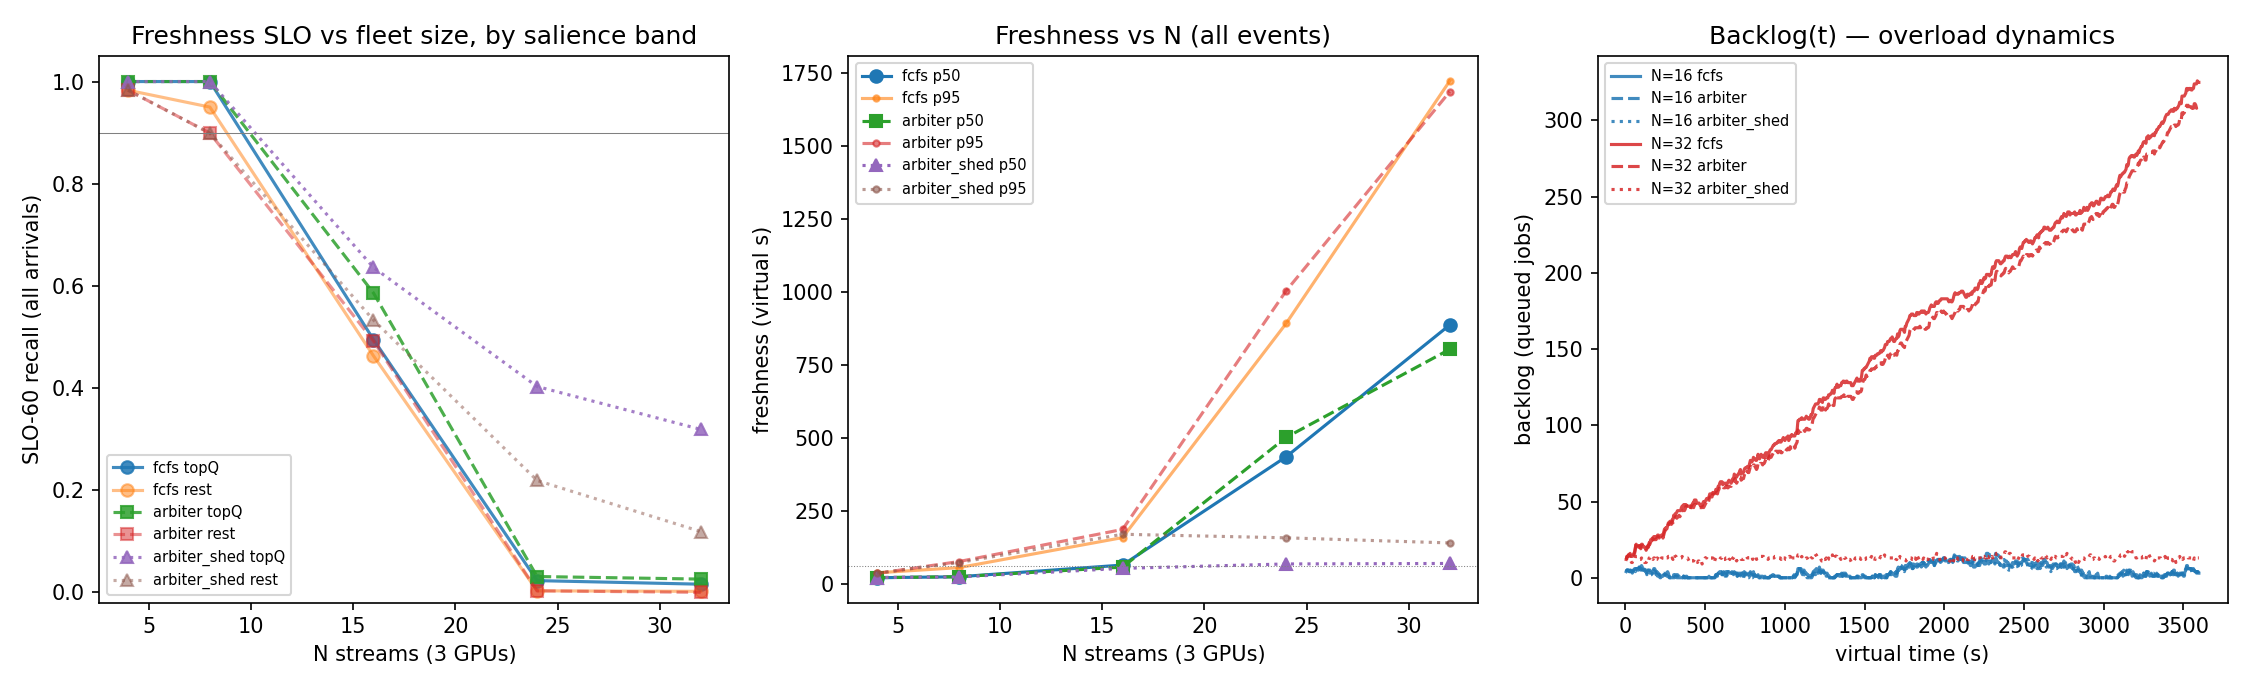
\includegraphics[width=\columnwidth]{figures/fleet_v1_curves.png}
\caption{Fleet v1: SLO-60 recall vs.\ fleet size per policy, split by salience band; backlog traces confirm the admission-control mechanism.}
\label{fig:fleet}
\end{figure}

\subsection{Eviction under a storage budget}
\label{sec:exp-eviction}

We sweep retention $\in \{50, 25, 10, 5, 2\}\%$ of the full-corpus memory (749 events) under five policies --- recency (FIFO), random, salience-only, coverage (ours), coverage+tombstones --- and re-run the 220 SMB queries per cell (36 cells; no new inference).

\begin{table}[t]
\centering
\caption{Eviction frontier, corrected reporting (61-cell matrix: policy $\times$ tombstones $\times$ budget; random = mean of 3 seeds). Existence accuracy is reported alone --- it collapses under eviction and balanced accuracy hides this (negation FAR mechanically falls as memory shrinks). Tombstones lift \emph{only} retrieval AP; with tombstones ON, all policies converge (AP 0.173--0.184 at 2\%), i.e., the stubs, not the selection, carry the aggregate signal.}
\label{tab:eviction}
\small
\begin{tabular}{@{}lcccc@{}}
\toprule
Policy & Existence @25\% & AP @25\% (OFF$\to$ON) & AP @10\% (OFF$\to$ON) & AP @2\% (OFF$\to$ON) \\
\midrule
None (100\%) & \textbf{0.950} & \multicolumn{3}{c}{AP 0.353 (no eviction)} \\
\midrule
Recency (FIFO) & 0.183 & .163 $\to$ .178 & .077 $\to$ .125 & .047 $\to$ \textbf{.184} \\
Salience & 0.283 & .177 $\to$ .200 & .074 $\to$ .118 & .052 $\to$ \textbf{.184} \\
Coverage (ours) & \textbf{0.333} & .091 $\to$ .162 & .053 $\to$ .122 & .027 $\to$ .173 \\
Random & 0.350 & .148 $\to$ .182 & .066 $\to$ .116 & .044 $\to$ .176 \\
\bottomrule
\end{tabular}
\end{table}

Findings (Figure~\ref{fig:eviction}): (i) \textbf{point queries collapse under eviction regardless of policy} --- existence accuracy falls from 0.950 to 0.18--0.35 at 25\% retention, a fact our earlier balanced-accuracy reporting had hidden (the negation-FAR confound); (ii) without tombstones, selection policy matters for breadth --- coverage retains the most rare events (GT coverage 0.352 vs.\ recency's 0.302 at 25\%) and the best balanced accuracy; (iii) \textbf{tombstones rescue aggregate answerability but equalize policies}: retrieval AP at 2\% retention rises 3.5$\times$ against the strongest selection policy (salience, 0.052$\to$0.184) and 6.4$\times$ against the weakest (coverage, 0.027$\to$0.173), with all policies converging to 0.173--0.184 --- eviction as compression works, but the compression, not the selection, does the work; (iv) the tombstone gain is budget-dependent: large at 2--10\%, negligible at 50\%.

\begin{figure}[t]
\centering
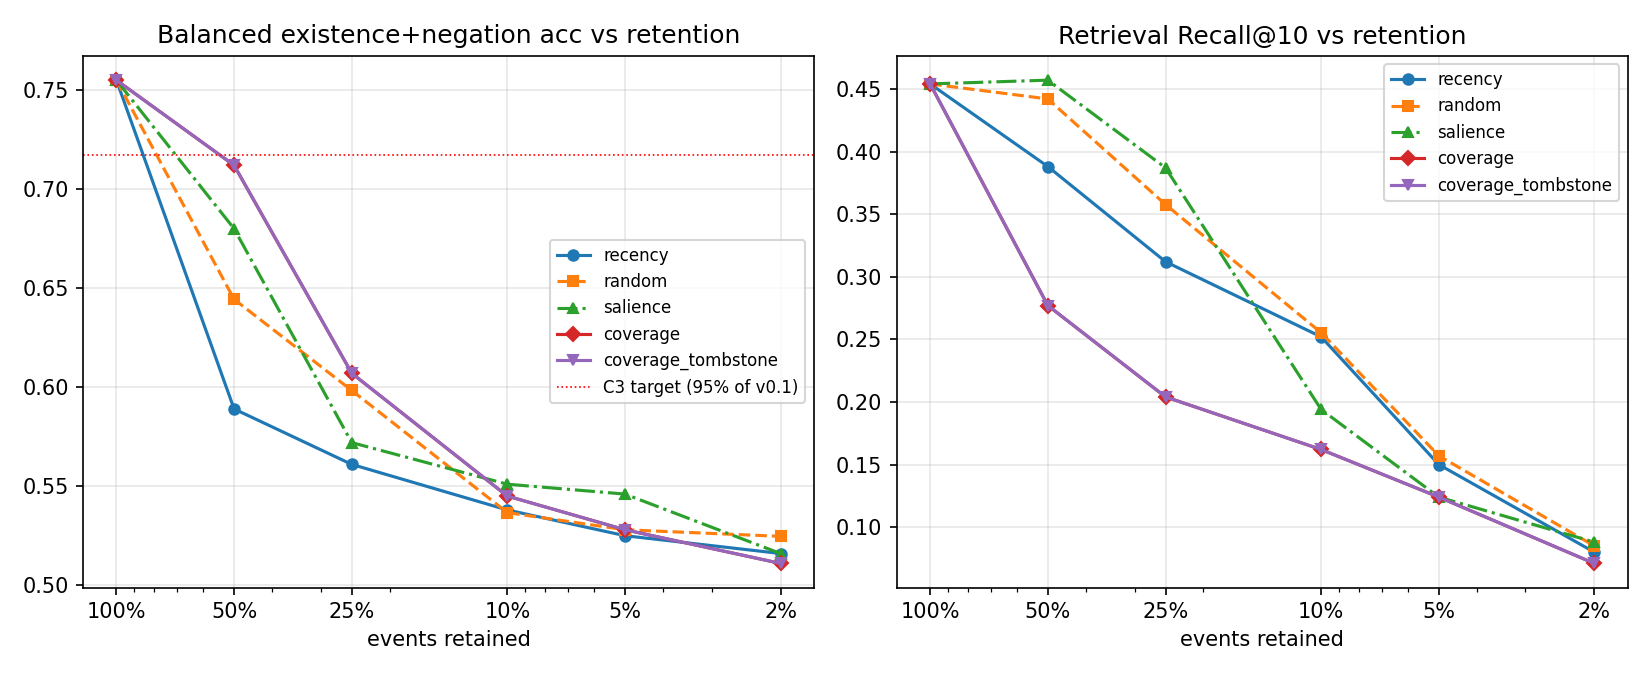
\includegraphics[width=\columnwidth]{figures/eviction_frontier.png}
\caption{Eviction frontier: query accuracy vs.\ retention budget per policy.}
\label{fig:eviction}
\end{figure}

\subsection{Appearance vs.\ event semantics: TASTI-lite}
\label{sec:exp-tasti}

TASTI-lite instantiates the classical semantic index in our setting: CLIP ViT-B/16 embeddings~\cite{clip} of 4{,}944 uniform 30-s chunks, text-encoder queries, threshold calibrated on the same frozen split, identical metrics code. It is deliberately given more raw coverage than \sys (every chunk embedded).

\begin{table}[h]
\centering
\caption{Appearance-only memory vs.\ text+tag memory (same 220 queries). The E0 appearance-signature finding holds in-system.}
\label{tab:tasti}
\small
\begin{tabular}{@{}lcc@{}}
\toprule
 & TASTI-lite & \sys v0.1 \\
\midrule
Existence acc & 0.583 & \textbf{0.950} \\
Negation FAR & \textbf{0.200} & 0.440 \\
Temporal tIoU & 0.167 & \textbf{0.286} \\
Retrieval R@10 / AP & 0.269 / 0.157 & \textbf{0.454 / 0.353} \\
\bottomrule
\end{tabular}
\end{table}

Appearance embeddings lack event semantics (Table~\ref{tab:tasti}) --- the same conclusion our cross-camera analysis reached offline (label agreement 0.55--0.59 vs.\ 0.501 chance; Appendix~\ref{app:e0}) --- now demonstrated in a running system. Its only win (negation FAR 0.20) is mechanical: an under-triggering index false-alarms less.

\subsection{Generality: beyond surveillance}
\label{sec:exp-generality}

To test whether the write-cost principle is surveillance-specific, we run RVS-Ego (ReKV's native benchmark) with three systems: ReKV-0.5B, uniform captioning, and \emph{novelty-gated writes} --- \sys's ladder with a domain-neutral CLIP-delta gate in place of the anomaly signal.

\begin{table}[h]
\centering
\caption{Generality arm (RVS-Ego, 120 questions, token-F1; GPT-judge unreachable offline --- relative comparison only). The gating principle generalizes; caption memory is lossy for fine-grained procedural QA (Section~\ref{sec:discussion}).}
\label{tab:generality}
\small
\begin{tabular}{@{}lccc@{}}
\toprule
System & token-F1 & Write GPU-s/stream-h & GPU-s/query \\
\midrule
ReKV-0.5B (native) & \textbf{0.212} & 341 & 0.88 \\
Uniform writes & 0.143 & 851 & 0.91 \\
Novelty-gated (ours) & 0.130 & \textbf{418} & 0.88 \\
\bottomrule
\end{tabular}
\end{table}

The event-driven write principle transfers (half the write cost of uniform at comparable accuracy, no domain model); the caption representation does not dominate on fine-grained procedural QA, where full-fidelity KV retrieval wins. Section~\ref{sec:discussion} draws the design conclusion (a hybrid memory with an optional KV tier).
